\documentclass[12pt]{article}

\usepackage{booktabs}
\usepackage{dcolumn} 
\usepackage{epstopdf}
\usepackage{graphicx}
\usepackage{hyperref}
\usepackage{longtable} 
\usepackage{natbib}
\usepackage{rotating}
\usepackage{tabularx}
\usepackage{amsmath}
\usepackage{setspace}
\usepackage{caption}
\usepackage{epigraph}

\usepackage[super]{nth}  
\hypersetup{
  colorlinks = TRUE,
  citecolor=blue,
  linkcolor=red,
  urlcolor=black
}

\hypersetup{colorlinks = TRUE, citecolor=blue, linkcolor=red, urlcolor=black}

\DeclareMathOperator*{\argmax}{arg\,max}

\newcommand{\starlanguage}{Significance indicators: $p \le 0.1:*$, $p \le 0.05:**$ and $p \le .01:***$.}

\newcommand{\covid}{COVID-19}  

\newtheorem{proposition}{Proposition}
\newtheorem{assumption}{Assumption}
\newtheorem{example}{Example}
\newtheorem{observation}{Observation}
\newtheorem{lemma}{Lemma}

\newcommand{\important}[1]{\textcolor{blue}{\textbf{ #1}}}
\newcommand{\quantclaim}[1]{\textcolor{red}{\textbf{ #1}}}


\newcommand{\LFPRhat}{58}
\newcommand{\numObs}{4,946}
\newcommand{\numObsWorking}{2,845}
\newcommand{\SurveyStart}{2020-06-29}
\newcommand{\SurveyEnd}{2020-07-04}
\newcommand{\LaidOff}{8.0}
\newcommand{\LaidOffLB}{4.5}
\newcommand{\LaidOffUB}{11.5}
\newcommand{\WFH}{28.4}
\newcommand{\WFHLB}{25.3}
\newcommand{\WFHUB}{31.5}
\newcommand{\alreadyWFH}{14.3}
\newcommand{\alreadyWFHLB}{10.9}
\newcommand{\alreadyWFHUB}{17.7}
\newcommand{\stillCommute}{42.7}
\newcommand{\stillCommuteLB}{40.0}
\newcommand{\stillCommuteUB}{45.5}


\begin{document} 



\title{COVID-19 and Remote Work:\\ An Early Look at US Data\footnote{
    MIT's COUHES ruled this project exempt (project number E-2075).
    {Code \& Data: \href{https://github.com/johnjosephhorton/remote\_work/}{https://github.com/johnjosephhorton/remote\_work/}}.
    Thanks to Sam Lord for helpful comments. 
  }}

\date{\today}

\date{\today}

\author{Erik Brynjolfsson\\MIT, Stanford \& NBER \and John Horton\\MIT \& NBER \and Adam Ozimek\\Upwork \and Daniel Rock\\MIT \and Garima Sharma\\MIT \and Hong Yi Tu Ye\\MIT}


\maketitle

\begin{abstract}
  \noindent 
  We report the results of a nationally-representative sample of the US population on how they are adapting to the \covid{} pandemic.
  The survey ran from May 2-8, 2020.
  Of those employed four weeks earlier, \WFH{}\% report they were commuting and are now working from home.
  In addition, \LaidOff{}\% report being laid-off or furloughed in the last 4 weeks. There is a strong negative relationship between the fraction in a state still commuting to work and the fraction working from home which suggests that many workers currently commuting could be converted to remote workers.  We find that the share of people switching to remote work can be predicted  by the incidence of \covid{} and that younger people were more likely to switch to remote work.  States with a higher share of employment in management, professional and related occupations were more likely to experience large shifts toward working from home and had fewer people laid off or furloughed.
  Furthermore, using data on state unemployment insurance (UI) claims, we find that states with higher fractions of remote workers have higher-than-expected UI claims. A prior version of the survey ran from April 1-5, 2020, and we find no substantial change in results between the two waves, suggesting that most changes to remote work manifested by early April.
  \newline 
\end{abstract} 

\onehalfspacing 

\section{Introduction}
The on-going \covid{} pandemic is rapidly transforming how, and even whether, people work. It has confined large numbers of people to their homes via quarantines and shelter-in-place orders. Large numbers of businesses are closed and many people are not working remotely. There have already been enormous and unprecedented increases in workers filing unemployment insurance claims \citep{goldsmith2020}. Whether or not any particular set of changes in work and employment lasts beyond the end of the pandemic, it is important to get a sense of where we are now.

To get a real-time sense of how firms and workers are responding, we conducted two waves of surveys using Google Consumer Surveys (GCS), one each in April and May.\footnote{
GCS is a relatively low-cost tool for rapidly collecting responses to simple questions \cite{stephens2014hands}, and response representativeness is often comparable to similar alternatives \citep{santoso2016survey, brynjolfsson2019using}.}  In the April version of the survey we asked a single question:
````Have you started to work from home in the last 4 weeks?''
with the following response options: 
\begin{enumerate} 
\item ``I continue to commute to work''
\item ``I have recently been furloughed or laid-off''
\item ``Used to commute, now work from home''   
\item ``Used to work from home and still do''       
\item ``Used to work from home, but now I commute''
\item ``None of the above / Not working for pay''
\end{enumerate} 
In the May version, we updated the question to: ````Have you started to work from home in the last 2 months?''

We launched a first wave of our survey on April 1, 2020 and collected responses until April 5, collecting a total of \numObsold{} responses. We launched a second wave on May 2, 2020, collecting \numObs{} responses until May 8, 2020. We find across both waves that over one third of workers have responded to the pandemic by shifting to remote work, while another 10\% have been laid-off or furloughed.
There is a great deal of variation across states in the share of people switching to remote work as well the share of people who continue to commute. We find that these can each be predicted by incidence of COVID-19 as well as the industry composition of the state prior to the crisis' onset.  We also find that younger people were more likely than older people to switch from commuting to remote work. Responses did not meaningfully differ across the two survey waves, suggesting that most changes to remote work had already manifested by early April. We therefore report results from the May version of the survey in the main figures, and explore across-time differences in Section 2.5 below. 

\section{Results}
We report results from Wave 2 (May) of the survey, noting in section 2.5 below that responses did not vary meaningfully across the waves. Of the respondents, \numObsWorking{} reported something other than ``None of the above...''
This gives an implied employment rate of \LFPRhat{}\%, which is slightly lower than the BLS estimate of about 60\%.\footnote{
  \url{https://fred.stlouisfed.org/series/EMRATIO}
}
For the rest our analysis, we restrict our sample to those reporting being employed four weeks prior.

The distribution of answers pooled over all respondents is shown in Figure~\ref{fig:working_summary}. 
We can see that the most common response from workers was that they continue to commute, at \stillCommute{}\% (95\% CI is [\stillCommuteLB,\stillCommuteUB]). 
But the next most common was that they have switched from commuting to working from home. 

The fraction of workers who switched to working from home is about \WFH{}\%.  In addition,  \alreadyWFH{}\% reporting they were already working from home pre-COVID-19.  This suggests nearly half the workforce is now working from home, significantly more than the \cite{dingel2020} estimate of 37\% of people working at home.\footnote{
Our estimates are broadly consistent with the literature, however there is a relatively wide range of estimates.
\cite{krantz2019did} uses 2013-2017 American Time Use Survey (ATUS) data to show 20.5\% of workers working from home in some way on an average day.
However, our question implies working from home all the time.
The remote worker fraction in the ATUS is 11.4\%.
Our 14.2\% estimate is also broadly consistent with the ``Freelancing in America Survey'' that reported 16.8\% of workers report doing most or all of their work remotely, though this includes people working from co-working spaces, coffee shops, homes, etc \citep{ozimek2020}.
At the lowest end, the 2019 Census reports 5.3\% of workers as ``working from home.''
The wide range in answers suggests respondent uncertainty about the precise meaning of questions. Nevertheless, our results lie well within the existing estimates.
}

% NEED TO FIX THIS PARAGRAPH. TOTAL INITIAL UI CLAIMS ARE 30MILLION SINCE THE START OF APRIL.
We find that \LaidOff{}\% of workers report recently being laid off or furloughed. If we take the US labor force at about 165 million, this implies that about 16.5 million Americans are recently out of work.
The total new UI filings for the last six weeks add up to 30 million, suggesting our survey offers an underestimate of the fraction laid off.\footnote{
  \url{https://www.dol.gov/ui/data.pdf}
}

\begin{figure}
  \caption{Answers to the question ``Have you started to work from home in the last 2 months?'', conditional upon being in the labor force from a US sample} \label{fig:working_summary}
\centering
\begin{minipage}{1.1 \linewidth}
  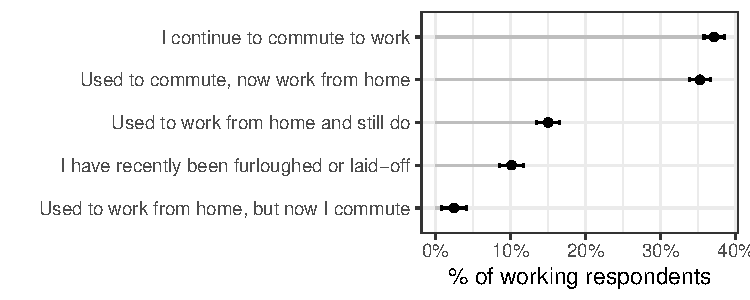
\includegraphics[width = \linewidth]{plots/working_summary.pdf} \\
  \begin{footnotesize}
    %% \begin{singlespace}
    %%   \emph{Notes:} 
    %% \end{singlespace}
    \end{footnotesize}
\end{minipage}
\end{figure} 

\subsection{Geographic variation} 
COVID-19 has affected various parts of the US differently, with the main epicenter in New York City.
In Figure~\ref{fig:region}, we plot the fraction of respondents choosing each answer by region.
GCS captures a respondent's city and state, which are then mapped to the regions ``Northeast'', ``Midwest'', ``West'', and ``South.'' 

In the first facet from the left, we can see that the South has the highest fraction still commuting to work and the Northeast has the lowest. 
In the second facet from the right, we can see that the Northeast has the highest fraction of respondents switching to working from home, and the South has the fewest.
The Northeast started from the lowest fraction working from home, though these fractions are imprecisely estimated and are all fairly similar to each other. 
The Northeast fraction now working from home is over 40\%. 

\begin{figure}
  \caption{Responses by US region} \label{fig:region}
\centering
\begin{minipage}{1.0 \linewidth}
  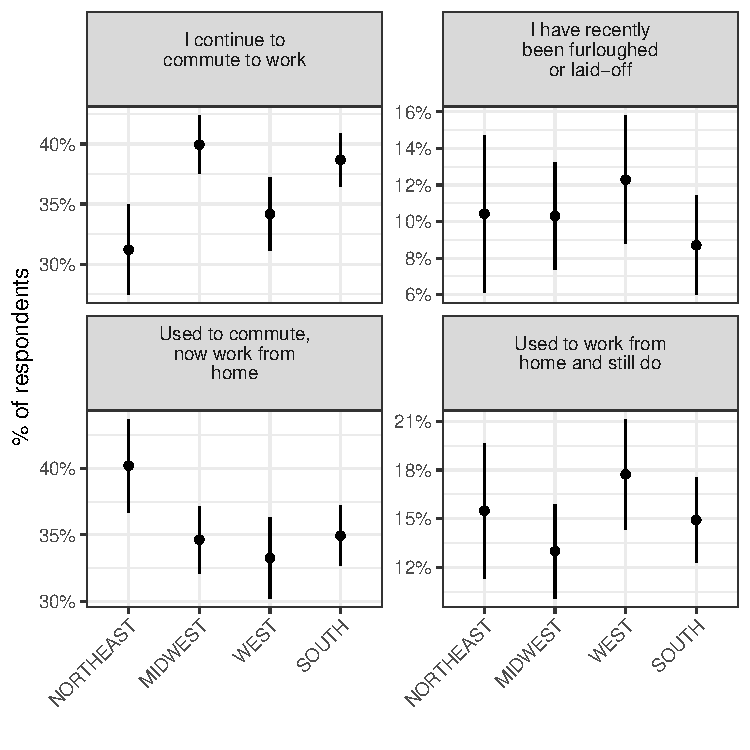
\includegraphics[width = \linewidth]{plots/region.pdf} \\
  \begin{footnotesize}
%    \begin{singlespace}
%      \emph{Notes:} Standard errors are reported. 
%    \end{singlespace}
    \end{footnotesize}
\end{minipage}
\end{figure} 

For a finer-grained look, we plot responses by state.
In Figure~\ref{fig:geo_wfh} we plot the fraction of respondents that switched to working remotely. 
As we saw in Figure~\ref{fig:region}, the highest fractions now working from home are in the Northeast.
The South and parts of the Midwest show substantially less remote work. 
%.\footnote{
%  We provide larger maps for each fraction in Appendix~\ref{sec:maps}. 
%}
It is important to keep in mind that some of these point estimates are fairly imprecise.


\subsection{By gender and age} \label{sec:gender}

In Figure~\ref{fig:gender} we report responses by inferred gender.
Fractions are computed separately for males and females, and then a slope graph is used to show differences. Within all questions at a 95\% confidence interval, the differences between gender are not statistically significant. Within our sample, however, it appears that men were modestly more likely to continue to commute to work, and likewise women more were more likely to report switching from commuter to work from home status. Men were also slightly more likely to have been recently furloughed or laid-off. Consistently working from home workers show little different in gender composition.

\begin{figure}
  \caption{Responses by gender} \label{fig:gender}
\centering
\begin{minipage}{1.0 \linewidth}
  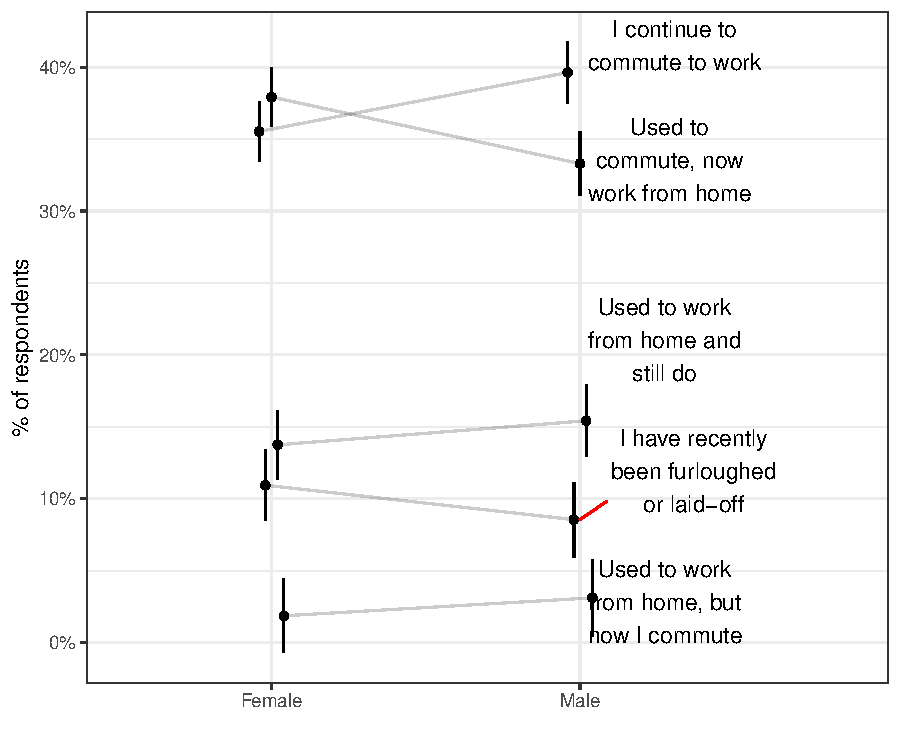
\includegraphics[width = \linewidth]{plots/gender.pdf} \\
  \begin{footnotesize}
    \begin{singlespace}
 %     \emph{Notes:} Standard errors are reported. 
    \end{singlespace}
    \end{footnotesize}
\end{minipage}
\end{figure} 


In Figure~\ref{fig:by_age} we report responses by inferred age.
A similar proportion of workers continue to commute to work across all age groups, as is also the case for the recently furloughed or laid-off worker contingent.
On the other hand, the proportion of respondents that has recently converted from commuting to work to remote work steadily declines from the 25-34 age group to the 65 and older category. The differences between the 25-34 age group and the 65 and older group are statistically significant, and, as Figure~\ref{fig:by_age} shows, younger workers (above age 25) are more likely to have been converted to work from home from commuting. 

Survey respondents in older age groups also reported \emph{remaining} working remotely with greater propensities.
These results are directionally consistent with the 2019 Census~\cite{ACSTableB08101}, though our estimates are larger.
The differences may arise from a difference in the question asked.
The Census asks about how workers get to work. The 2019 Upwork ``Freelancing in America'' study found younger workers were modestly \emph{more} likely to work mostly or entirely from home~\cite{upwork2019}.
It is possible that our survey is somewhere in between, grouping people who do some work at home with those who are fully committed remote labor.
We will investigate further in future work.

\begin{figure}
  \caption{Responses by inferred age} \label{fig:by_age}
\centering
\begin{minipage}{1.0 \linewidth}
  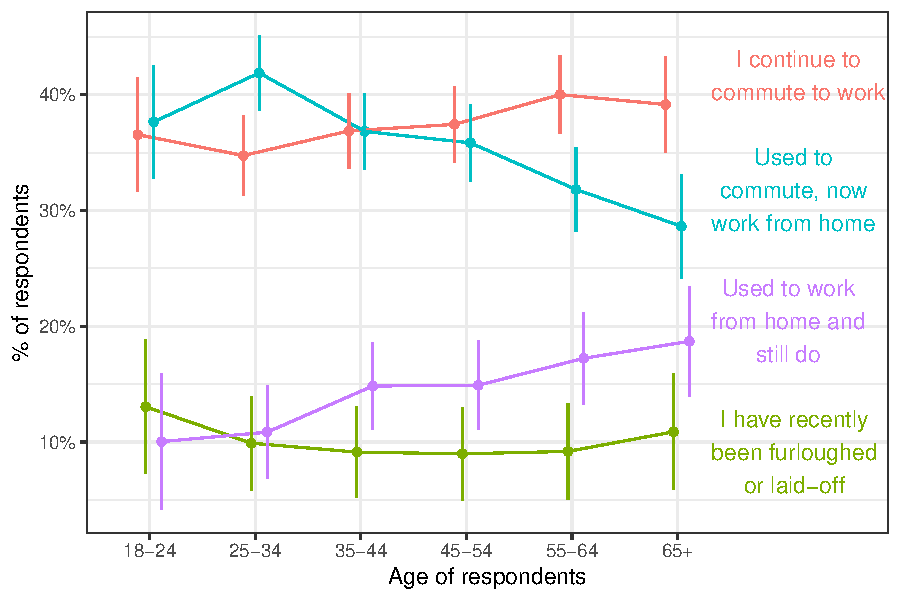
\includegraphics[width = \linewidth]{plots/by_age.pdf} \\
  \begin{footnotesize}
    \begin{singlespace}
 %     \emph{Notes:} Standard errors are reported. 
    \end{singlespace}
    \end{footnotesize}
\end{minipage}
\end{figure} 


%The fraction of workers that are still continuing to commute to work is highest in the Dakotas, Wyoming, and Montana.
%There is still a substantial fraction in the South continuing to commute. 
%The Northeast, with the exception of Vermont, shows large reductions in people still commuting to work. 

\begin{figure}
  \caption{Fraction now working remotely, by US State} \label{fig:geo_wfh}
\centering
\begin{minipage}{1.0 \linewidth}
  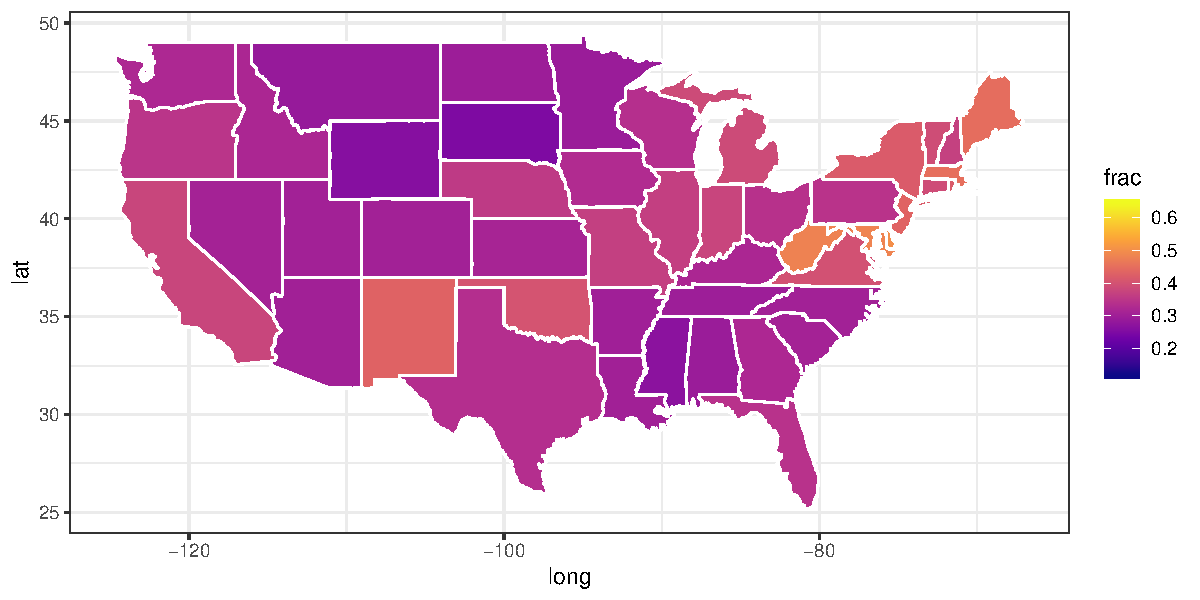
\includegraphics[width = \linewidth]{plots/geo_wfh.pdf} \\
  \begin{footnotesize}
    \end{footnotesize}
\end{minipage}
\end{figure} 

\subsection{Predictors of across-state variation} \label{sec:predictorsstate}
The fractions laid-off or furloughed by US State are shown in Figure~\ref{fig:geo_laidoff}.

\begin{figure}
  \caption{Fraction Laid-off/furloughed, by US State} \label{fig:geo_laidoff}
\centering
\begin{minipage}{1.0 \linewidth}
  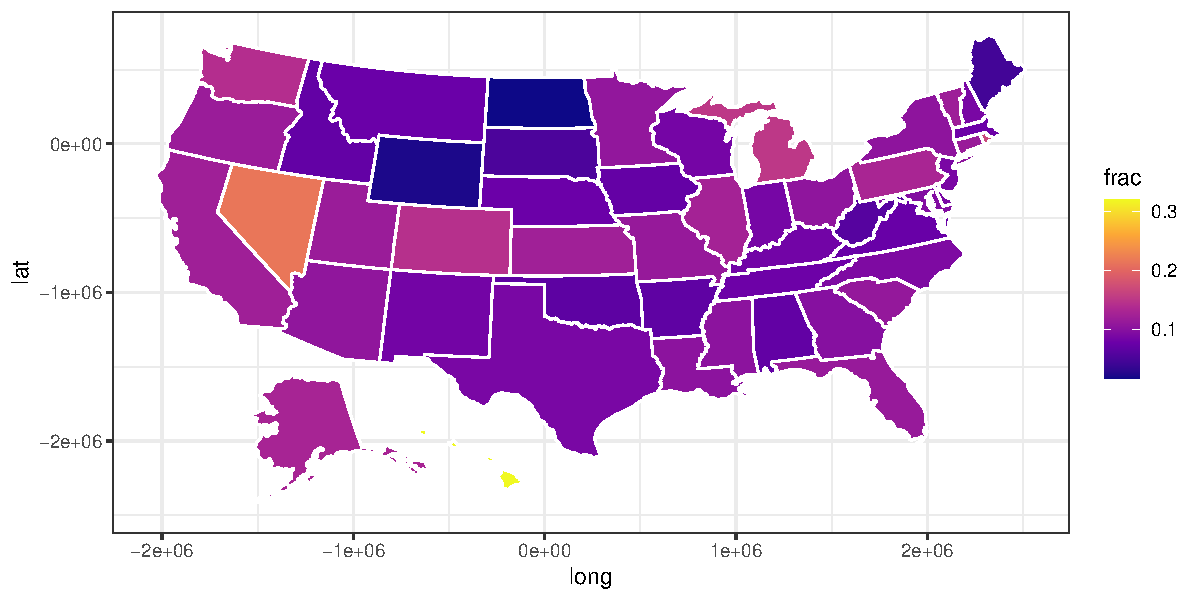
\includegraphics[width = \linewidth]{plots/geo_laidoff.pdf} \\
  \begin{footnotesize}
    \end{footnotesize}
\end{minipage}
\end{figure} 

In Figure~\ref{fig:commute_vs_wfh} we plot the fraction of respondents working from home versus the fraction still commuting by US state.
There is a clear negative relationship, suggesting a fraction of current commuters could potentially transition to work-from-home status.
Each 10 percentage point increase in the fraction still commuting is associated with about a 6 percentage point decline in the fraction of workers now working from home. 

\begin{figure}
  \caption{Still commuting versus work from home fractions by US State} \label{fig:commute_vs_wfh}
\centering
\begin{minipage}{0.8 \linewidth}
  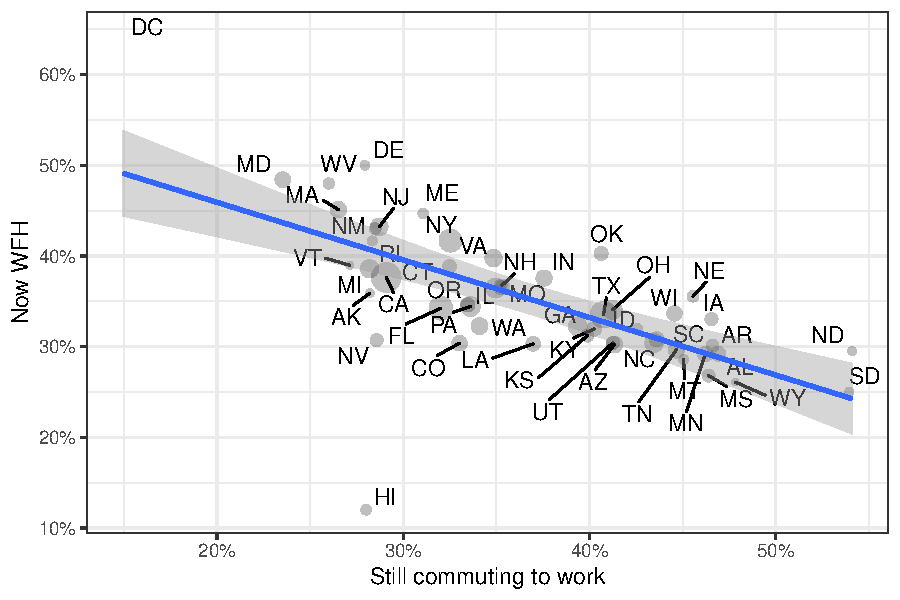
\includegraphics[width = \linewidth]{plots/commute_vs_wfh.pdf} \\
  \begin{footnotesize}
    %% \begin{singlespace}
    %%   \emph{Notes:} 
    %% \end{singlespace}
    \end{footnotesize}
\end{minipage}
\end{figure} 

Table~\ref{tab:remotework} documents how heterogeneity in COVID infection rates (measured as the log of cases per 100,000 individuals\footnote{Data accessed on May 16, 2020 from The New York Times: https://github.com/nytimes/covid-19-data}) affects switching to remote work or continuing to work from home. We report results from the April (wave 1) as well as May (wave 2) waves of the survey. Column (1) shows that a 100\% rise in COVID-19 cases per 100k individuals is associated with a 5\% rise in the fraction of workers who switch to working from home in wave 1 and a 4.3\% rise in wave 2. Column (2) shows a similar rise in COVID-19 incidence as predicting a 5.4\% fall in the fraction of those continuing to commute in wave 1, and 2.7\% in wave 2. Waves 1 and 2 show remarkable consistency, supporting the conclusion that most changes to remote work occurred by the first wave. We would expect these relationships if higher spread is associated with higher responsiveness of government or individuals. Surprisingly, we do not find a strong or statistically significant relationship between our measure of incidence and survey reports of being furloughed or laid-off. These associations are not to be interpreted as causal and future work will explore the causal effect of the pandemic on switches into remote work.

\begin{table}[!htbp] \centering                    \caption{Predicting remote work by state incidence of COVID-19}                    \label{tab:remotework}                  \small                  \begin{tabular}{@{\extracolsep{5pt}}lccc}                  \\[-1.8ex]\hline                  \hline \\[-1.8ex]                   & \multicolumn{3}{c}{\textit{Dependent variable:}} \\                   \cline{2-4}                   \\[-1.8ex] & Work from home & Continue to commute & Furloughed or laid-off \\                   \hline \\[-1.8ex]               
                    &\multicolumn{1}{c}{(1)}         &\multicolumn{1}{c}{(2)}         &\multicolumn{1}{c}{(3)}         \\
\hline \\               & \multicolumn{3}{c}{\textit{Panel A: Wave 1}} \\               \addlinespace[1mm] \\
Log cases per 100k  &       0.050\sym{***}&      -0.054\sym{***}&      -0.000         \\
population          &     (0.012)         &     (0.015)         &     (0.007)         \\
[1em]
Constant            &       0.136\sym{***}&       0.590\sym{***}&       0.122\sym{***}\\
                    &     (0.047)         &     (0.059)         &     (0.028)         \\
[1em]
Observations        &          51         &          51         &          51         \\
\(R^{2}\)           &        0.23         &        0.19         &        0.00         \\

\hline \\               & \multicolumn{3}{c}{\textit{Panel B: Wave 2}} \\               \addlinespace[1mm] \\
Log cases per 100k  &       0.043\sym{***}&      -0.027\sym{*}  &      -0.004         \\
population          &     (0.015)         &     (0.014)         &     (0.011)         \\
[1em]
Constant            &       0.115         &       0.513\sym{***}&       0.124\sym{*}  \\
                    &     (0.083)         &     (0.079)         &     (0.067)         \\
[1em]
Observations        &          51         &          51         &          51         \\
\(R^{2}\)           &        0.22         &        0.07         &        0.01         \\
\hline                         \hline                          \hline \\[-1.8ex]                          \end{tabular}                         \\                         \begin{minipage}{1.0 \textwidth}                         {\footnotesize \emph{Notes}:                          \starlanguage}                         \end{minipage}                         \end{table}


Tables~\ref{tab:priorremotework}, ~\ref{tab:priorindustry}, and ~\ref{tab:priorindustrymanuf} document how the pre-COVID distribution of economic activity across states predicts shifts into remote work. In Table~\ref{tab:priorremotework} we look at how the pre-COVID share of workers working from home (measured in the 2017 ACS) influences survey responses.  Interestingly, pre-COVID work from home share is not strongly predictive of COVID-induced shares of people working from home or continuing to commute in either of the two survey waves. 

\begin{table}[!htbp] \centering                    \caption{Predicting remote work by pre COVID-19 work from home}                    \label{tab:priorremotework}                  \small                  \begin{tabular}{@{\extracolsep{5pt}}lccc}                  \\[-1.8ex]\hline                  \hline \\[-1.8ex]                   & \multicolumn{3}{c}{\textit{Dependent variable:}} \\                   \cline{2-4}                   \\[-1.8ex] & Work from home & Continue to commute & Furloughed or laid-off \\                   \hline \\[-1.8ex]               
                    &\multicolumn{1}{c}{(1)}         &\multicolumn{1}{c}{(2)}         &\multicolumn{1}{c}{(3)}         \\
\hline \\               & \multicolumn{3}{c}{\textit{Panel A: Wave 1}} \\               \addlinespace[1mm] \\
Pre-COVID fraction  &       1.161         &      -1.464         &      -0.325         \\
working from home   &     (0.915)         &     (1.357)         &     (0.524)         \\
[1em]
Constant            &       0.278\sym{***}&       0.445\sym{***}&       0.136\sym{***}\\
                    &     (0.040)         &     (0.061)         &     (0.026)         \\
[1em]
Observations        &          51         &          51         &          51         \\
\(R^{2}\)           &        0.02         &        0.02         &        0.01         \\
\hline \\               & \multicolumn{3}{c}{\textit{Panel B: Wave 2}} \\               \addlinespace[1mm] \\
Pre-COVID fraction  &       0.337         &      -1.057         &      -0.038         \\
working from home   &     (0.974)         &     (1.006)         &     (0.441)         \\
[1em]
Constant            &       0.337\sym{***}&       0.416\sym{***}&       0.103\sym{***}\\
                    &     (0.044)         &     (0.047)         &     (0.023)         \\
[1em]
Observations        &          51         &          51         &          51         \\
\(R^{2}\)           &        0.00         &        0.02         &        0.00         \\
\hline                         \hline                          \hline \\[-1.8ex]                          \end{tabular}                         \\                         \begin{minipage}{1.0 \textwidth}                         {\footnotesize \emph{Notes}:                          \starlanguage}                         \end{minipage}                         \end{table}


In contrast, Table~\ref{tab:priorindustry} shows not all occupations have been affected equally.  In particular, states with more workers in ``management, professional and related occupations" (\cite{krantz2019did}) were more likely to have large shifts into remote work. This is consistent with the classification of these occupations by the Bureau of Labor Statistics as having high potential for working from home. Columns (1)-(2) show that, in the April wave of the survey, a 1\% rise in the share of workers in these occupations is associated with a 1.1\% rise in those reporting now working from home and 1.1\% decline in those reporting that they continue to commute to work. The May wave yields similar numbers at 1.1\% rise in those reporting now working from home and a 0.9\% decline in those continuing to commute. Column (3) also shows a greater share in these occupations as being associated with a decline in furloughs or layoffs. 

\begin{table}[!htbp] \centering                    \caption{Management, Professional, and Related Occupations}                    \label{tab:priorindustry}                  \small                  \begin{tabular}{@{\extracolsep{5pt}}lccc}                  \\[-1.8ex]\hline                  \hline \\[-1.8ex]                   & \multicolumn{3}{c}{\textit{Dependent variable:}} \\                   \cline{2-4}                   \\[-1.8ex] & Work from home & Continue to commute & Furloughed or laid-off \\                   \hline \\[-1.8ex]               
                    &\multicolumn{1}{c}{(1)}         &\multicolumn{1}{c}{(2)}         &\multicolumn{1}{c}{(3)}         \\
\hline \\               & \multicolumn{3}{c}{\textit{Panel A: Wave 1}} \\               \addlinespace[1mm] \\
MPR share         &       1.152\sym{***}&      -1.100\sym{***}&      -0.229\sym{**} \\
&     (0.122)         &     (0.170)         &     (0.092)         \\
[1em]
Constant            &      -0.092\sym{*}  &       0.781\sym{***}&       0.205\sym{***}\\
                    &     (0.049)         &     (0.064)         &     (0.035)         \\
[1em]
Observations        &          51         &          51         &          51         \\
\(R^{2}\)           &        0.47         &        0.30         &        0.07         \\
\hline \\               & \multicolumn{3}{c}{\textit{Panel B: Wave 2}} \\               \addlinespace[1mm] \\
MPR share         &       1.076\sym{***}&      -0.889\sym{***}&      -0.143         \\
&     (0.126)         &     (0.164)         &     (0.119)         \\
[1em]
Constant            &      -0.043         &       0.694\sym{***}&       0.153\sym{***}\\
                    &     (0.050)         &     (0.066)         &     (0.048)         \\
[1em]
Observations        &          51         &          51         &          51         \\
\(R^{2}\)           &        0.45         &        0.28         &        0.02         \\
\hline                         \hline                          \hline \\[-1.8ex]                          \end{tabular}                         \\                         \begin{minipage}{1.0 \textwidth}                         {\footnotesize \emph{Notes}:                          \starlanguage}                         \end{minipage}                         \end{table}


Table~\ref{tab:priorindustrymanuf} shows that prior share in manufacturing employment is not a statistically significant predictor of switches into remote work. However, as expected, the sign of the coefficient is negative. Similarly, pre-COVID manufacturing share positively predicts continuing to commute. This pattern is statistically significantly different from zero in Wave 2 of the survey; a 1\% increase the pre-COVID share of employment in manufacturing is associated with a 0.84\% increase in continuing to commute to work.

\begin{table}[!htbp] \centering                    \caption{Manufacturing}                    \label{tab:priorindustrymanuf}                  \small                  \begin{tabular}{@{\extracolsep{5pt}}lccc}                  \\[-1.8ex]\hline                  \hline \\[-1.8ex]                   & \multicolumn{3}{c}{\textit{Dependent variable:}} \\                   \cline{2-4}                   \\[-1.8ex] & Work from home & Continue to commute & Furloughed or laid-off \\                   \hline \\[-1.8ex]               
                    &\multicolumn{1}{c}{(1)}         &\multicolumn{1}{c}{(2)}         &\multicolumn{1}{c}{(3)}         \\
\hline \\               & \multicolumn{3}{c}{\textit{Panel A: Wave 1}} \\               \addlinespace[1mm] \\
Mfg share       &      -0.151         &       0.549         &       0.070         \\
         &     (0.385)         &     (0.363)         &     (0.185)         \\
[1em]
Constant            &       0.347\sym{***}&       0.322\sym{***}&       0.114\sym{***}\\
                    &     (0.046)         &     (0.040)         &     (0.021)         \\
[1em]
Observations        &          51         &          51         &          51         \\
\(R^{2}\)           &        0.01         &        0.05         &        0.00         \\
\hline \\               & \multicolumn{3}{c}{\textit{Panel B: Wave 2}} \\               \addlinespace[1mm] \\
Mfg share        &      -0.346         &       0.838\sym{***}&      -0.113         \\
         &     (0.404)         &     (0.308)         &     (0.236)         \\
[1em]
Constant            &       0.387\sym{***}&       0.284\sym{***}&       0.112\sym{***}\\
                    &     (0.049)         &     (0.034)         &     (0.029)         \\
[1em]
Observations        &          51         &          51         &          51         \\
\(R^{2}\)           &        0.03         &        0.17         &        0.01         \\
\hline                         \hline                          \hline \\[-1.8ex]                          \end{tabular}                         \\                         \begin{minipage}{1.0 \textwidth}                         {\footnotesize \emph{Notes}:                          \starlanguage}                         \end{minipage}                         \end{table}


Taken together, these results suggest that places with greater capacity for increasing the amount of working from home are not necessarily places where workers are already working from home.  Instead, the occupation mix is more predictive than prior remote work of the ``remote-ability" of the marginal job that is not yet remote.

\subsection{Impact on UI claims} \label{sec:UI}

A natural question is how these various measures are affecting UI claims by state. 
In Table~\ref{tab:ui}, we combine our data with that on UI claims from the Bureau of Labor Statistics.

We regress the log of four weeks of UI claims in a state on the state's population and the log state-specific fraction for each of the response possibilities.  
Unsurprisingly, across all specifications, the state population explains a great deal of the variation in UI claims.
We are interested in asking whether our survey measures account for some of the residual variation.

To interpret these results, consider a state $i$ that has population $Pop_i$, an employment rate of $E_i$ and a COVID-induced fraction of the working population laid-off of $LO_i$. If UI claims perfectly measured lay-offs, then the state's UI claims would be $Pop_i E_i LO_i$ and so a regression of log UI claims on the log of each of the terms should give each component a coefficient on $1$. 
In the regressions in Table~\ref{tab:ui}, we use a state-specific employment rate pre-COVID calculated from our own survey and the state population. 

\begin{table}[!htbp] \centering                    \caption{Predicting UI claims by state}                    \label{tab:ui}                  \small                  \begin{tabular}{@{\extracolsep{5pt}}lcccc}                  \\[-1.8ex]\hline                  \hline \\[-1.8ex]                   & \multicolumn{4}{c}{\textit{Dependent variable:}} \\                  \cline{2-5}                  \\[-1.8ex] & \multicolumn{4}{c}{Log state six week UI claims} \\                  \\[-1.8ex] & (1) & (2) & (3) & (4)\\                  \hline \\[-1.8ex]               
 \\
[1em]
Log of state        &       1.012\sym{***}&       1.019\sym{***}&       1.013\sym{***}&       1.125\sym{***}\\
population          &     (0.035)         &     (0.042)         &     (0.033)         &     (0.061)         \\
[1em]
Log of LFPR         &      -0.554         &      -0.492         &       0.249         &       0.154         \\
                    &     (0.408)         &     (0.499)         &     (0.470)         &     (0.526)         \\
[1em]
Still commuting     &      -1.666\sym{***}&                     &                     &                     \\
frac. (log)         &     (0.473)         &                     &                     &                     \\
[1em]
Now WFH frac. (log) &                     &       0.671         &                     &                     \\
                    &                     &     (0.708)         &                     &                     \\
[1em]
Laid-off frac. (log)&                     &                     &       2.940\sym{***}&                     \\
                    &                     &                     &     (0.673)         &                     \\
[1em]
Still WFH (log)     &                     &                     &                     &      -0.004\sym{**} \\
                    &                     &                     &                     &     (0.002)         \\
[1em]
Constant            &      -2.304\sym{***}&      -3.221\sym{***}&      -2.765\sym{***}&      -4.052\sym{***}\\
                    &     (0.519)         &     (0.788)         &     (0.553)         &     (0.793)         \\
[1em]
Observations        &          51         &          51         &          51         &          51         \\
\(R^{2}\)           &        0.95         &        0.93         &        0.94         &        0.93         \\
\hline                  \hline \\[-1.8ex]                  \end{tabular}                 \\                 \begin{minipage}{1.0 \textwidth}                 {\footnotesize \emph{Notes}:                 \starlanguage}                 \end{minipage}                 \end{table}


In Column~(1), we append the state-specific fraction reporting that they were still commuting to work.
The higher the fraction reporting still commuting, the lower the UI claims for that state.
States that still have large numbers commuting to work should have fewer lay-offs, and so the coefficient on the fraction still commuting should be negative.

In Column~(2), the greater the fraction that reports working from home, the \emph{higher} the UI claims.
 The fraction working from home should, on the one hand, have a protective effect, keeping workers from filing for UI, but on other hand, a state with a high WFH fraction has likely had a particularly severe labor market shock, with many additional workers laid-off. 
What seems likely is that workers who would otherwise be continuing to commute to work are splitting into (a) work-from-home or (b) filing for UI.
As states impose further restrictions on mobility, we should be able to get a sense of the resulting increases in UI filings based on how many workers can be successfully transitioned to remote work. 

Surprisingly, Column~(3), which includes a direct measure of reported lay-offs has the ``right'' sign, but is large in magnitude.
Furthermore, our expectation is that the elasticity of UI claims to the number laid-off should be 1. 
% our unemployment numbers are really off...

%How much of this is due to Michigan - a potential outlier? Or other state-specific effects?

\subsection{Changes over time} \label{sec:timechanges}

Survey responses between the first wave (April 1-5) and second wave (May 2-8) of the survey do not demonstrate significantly different patterns, driven largely by strong positive correlations in responses. For example, when looking within states, the correlation in reports of workers having switched into remote work is 0.79; for continuing to commute to work, the correlation is 0.73, and for being laid off or furloughed it is 0.63. As expected, the tables above thus reveal no meaningful change in pattern over time of workers switching into remote work, continuing to commute, or being laid off or furloughed. An earlier version of the paper \footnote{Can be accessed at https://github.com/johnjosephhorton/remote_work/}, which plotted Figures 1-7 using data from the first wave, shows them as also revealing remarkably similar patterns. Taken together, these suggest that most short-term changes to remote work and commuting had already occurred by the first week of April. 

To gauge whether changes in employment are dynamically responding to the COVID crisis, we regress state-level changes in survey responses across the two survey waves on changes in state-level COVID incidence. Table~\ref{tab:deltacovid} reports results. Column (1) reveals that change in COVID incidence is mildly predictive of changes in switches into remote work. A 1 point change in log of COVID 19 cases per 100,000 individuals between April and May increases switches into remote work during this period by 2\%. Change in COVID incidence does not, however, appear to affect either continuing to commute or layoffs and furloughs.

\begin{table}[!htbp] \centering                    \caption{Predicting changes to work using changes to COVID}                    \label{tab:deltacovid}                  \small                  \begin{tabular}{@{\extracolsep{5pt}}lccc}                  \\[-1.8ex]\hline                  \hline \\[-1.8ex]                   & \multicolumn{3}{c}{\textit{Dependent variable:}} \\                   \cline{2-4}                   \\[-1.8ex] & Work from home & Continue to commute & Furloughed or laid-off \\                   \hline \\[-1.8ex]               
                    &\multicolumn{1}{c}{(1)}         &\multicolumn{1}{c}{(2)}         &\multicolumn{1}{c}{(3)}         \\
[1em]
Log change in COVID &      -0.001         &       0.019\sym{**} &      -0.005         \\
cases per 100k      &     (0.008)         &     (0.009)         &     (0.006)         \\
[1em]
Constant            &       0.028         &      -0.110\sym{**} &       0.004         \\
                    &     (0.044)         &     (0.051)         &     (0.033)         \\
[1em]
Observations        &          51         &          51         &          51         \\
\(R^{2}\)           &        0.00         &        0.07         &        0.01         \\
\hline                         \hline                          \hline \\[-1.8ex]                          \end{tabular}                         \\                         \begin{minipage}{1.0 \textwidth}                         {\footnotesize \emph{Notes}:                          \starlanguage}                         \end{minipage}                         \end{table}


\subsection{Implications and suggestions for future work}
These are a set of preliminary analyses of a rapidly-evolving crisis. We have documented some early shifts in the economy, and it remains to be seen if some of these changes are last beyond the end of the pandemic. For instance, once businesses and individuals invest in the fixed costs of remote work, including technology but perhaps more importantly in developing the necessary human capital and organizational processes, then they may decide to stay with the new methods.  Furthermore, the crisis has forced people to try out new approaches, some of which may be unexpectedly efficient or effective.  In either case, lasting changes from the crisis would be expected.  

Additional work to understand these changes is needed. Future research will address how state-specific occupational distributions will affect the share of labor performed by remote workers, as well as the impact of the occupational distribution on the UI system.  Long term changes may involve not only remote work, but also  the structure of industries and international trade. For example, tasks that can be done by remote workers may be more likely to be off-shored, as distance becomes less relevant. The tasks that comprise many occupations may be unbundled and re-bundled to separate those that require in-person presence at a business from those that can be done remotely.

Critical to those decisions made by employers are the productivity effects of remote work. More evidence is needed to evaluate the productivity changes induced by allowing work from home. Relatedly, what percentage of tasks can be done remotely and how does it vary across professions and industries? Can we also observe (and explain) heterogeneity across states? These task-specific questions will be the focus of our next round of surveys.

For the COVID-19 pandemic in particular, we are also interested in how the disease spreads differentially across types of jobs. Remote work is one way in which employers can protect both the health and job security of their employees.


%    \begin{itemize}
%    \item How are state-specific occupational %distributions affecting the share of workers able to perform remote work? And what effect does this have on the UI system? 
%    \item Are COVID-19 deaths/hospitalizations affecting the adoption of remote work down the distribution of occupations based upon their ``remote-ability''? What are the productivity implications of switching to remote work?
%    \item Can we predict how UI claims evolve in states based on how much of the workforce they can successfully shift to remote work? 
%    \item What percentage of tasks can be done remotely and how does it vary across professions and industries? Can we also observe (and explain) heterogeneity across states? These task-specific questions will be the focus of our next round of surveys. 
%    \end{itemize}



\section{Conclusion}
We document some early facts about how the US labor force is responding to COVID-19 pandemic.  In particular, we find that in the past four weeks over one third of the labor force has switched to remote work. The state-level COVID-19 infection rates predict these switches. Furthermore, states with more people in management, professional and related occupations were more likely to see large shifts toward working from home and had fewer people laid off or furloughed. 

If there is hysteresis as people learn new ways to work remotely and businesses reorganize, the pandemic-driven changes may portend more lasting effects on the organization of work.
We will continue to track changes to the nature of remote work, asking how pandemic-induced changes transform workplaces in the short and long-term. \\

\noindent The code and data for this project are here:
\href{https://github.com/johnjosephhorton/remote\_work/}{https://github.com/johnjosephhorton/remote\_work/}.


\newpage \clearpage
\bibliographystyle{aer}
\bibliography{remote_work.bib}







%% \subsection{Better looking maps} \label{sec:maps}

%% \begin{figure}
%%   \caption{Responses by US State} \label{fig:geo}
%% \centering
%% \begin{minipage}{1.0 \linewidth}
%%   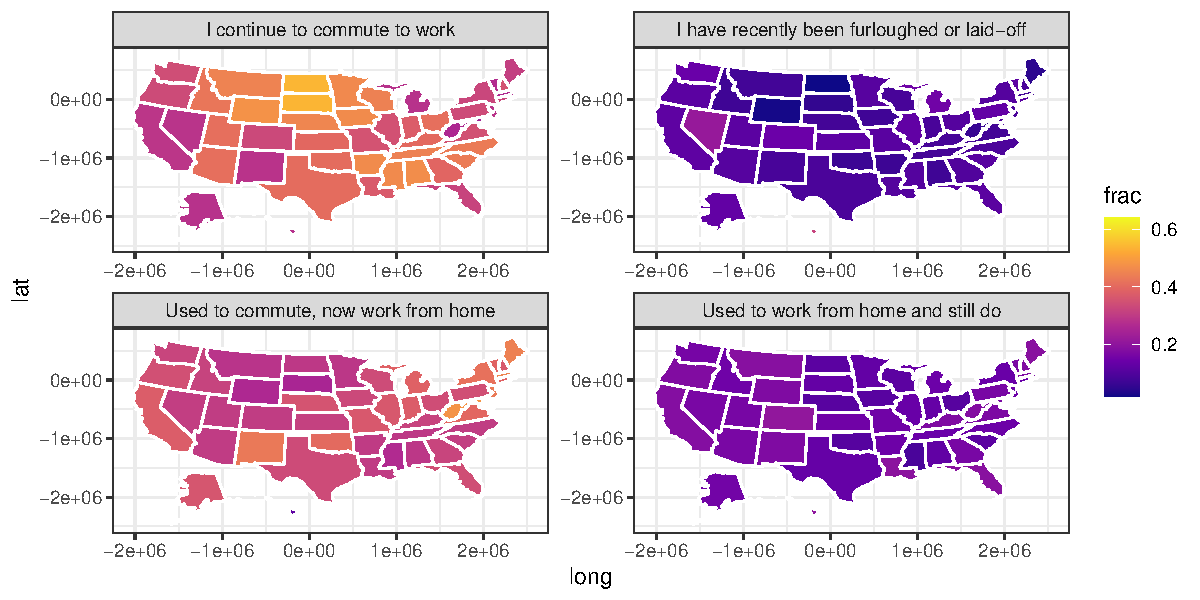
\includegraphics[width = \linewidth]{plots/geo.pdf} \\
%%   \begin{footnotesize}
%%     %% \begin{singlespace}
%%     %%   \emph{Notes:} 
%%     %% \end{singlespace}
%%     \end{footnotesize}
%% \end{minipage}
%% \end{figure} 

%% \begin{figure}
%%   \caption{Laid-off/furloughed by US State} \label{fig:gender}
%% \centering
%% \begin{minipage}{1.0 \linewidth}
%%   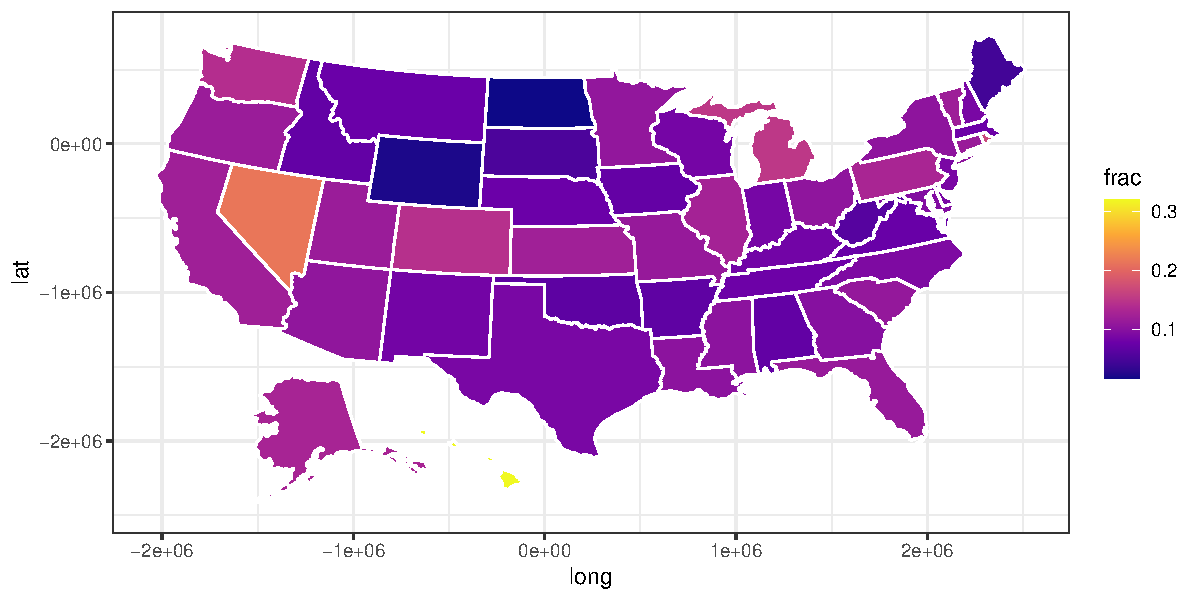
\includegraphics[width = \linewidth]{plots/geo_laidoff.pdf} \\
%%   \begin{footnotesize}
%%     \end{footnotesize}
%% \end{minipage}
%% \end{figure} 


%% \begin{figure}
%%   \caption{Now work-from-home by US State} \label{fig:wfh}
%% \centering
%% \begin{minipage}{1.0 \linewidth}
%%   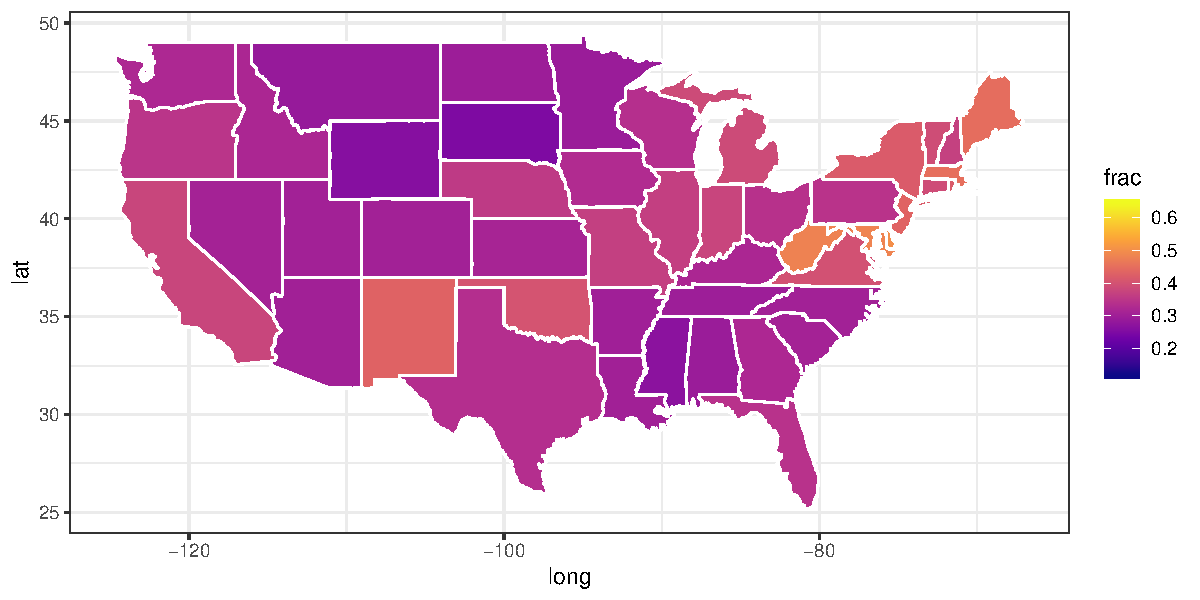
\includegraphics[width = \linewidth]{plots/geo_wfh.pdf} \\
%%   \begin{footnotesize}
%%     \end{footnotesize}
%% \end{minipage}
%% \end{figure} 

%% \begin{figure}
%%   \caption{Still commuting to work by US State} \label{fig:geo_still_commuting}
%% \centering
%% \begin{minipage}{1.0 \linewidth}
%%   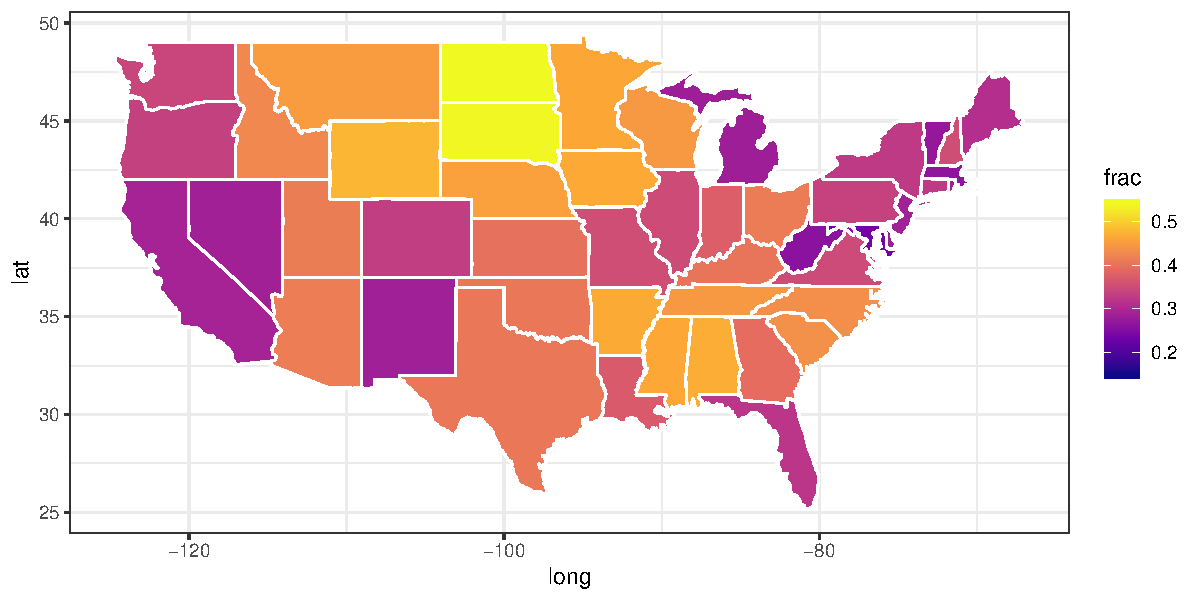
\includegraphics[width = \linewidth]{plots/geo_still_commuting.pdf} \\
%%   \begin{footnotesize}
%%     \end{footnotesize}
%% \end{minipage}
%% \end{figure} 


\end{document} 
